
% This is a Basic Assignment Paper but with like Code and stuff allowed in it. 

\documentclass[11pt]{article}

% Preamble

\usepackage[margin=1in]{geometry}
\usepackage{amsfonts, amsmath, amssymb}
\usepackage{fancyhdr, float, graphicx}
\usepackage[utf8]{inputenc} % Required for inputting international characters
\usepackage[T1]{fontenc} % Output font encoding for international characters
\usepackage{fouriernc} % Use the New Century Schoolbook font
\usepackage[nottoc, notlot, notlof]{tocbibind}
\usepackage{listings}
\usepackage{xcolor}
\usepackage{blindtext}
\usepackage{hyperref}
\hypersetup{
    colorlinks=true,
    linkcolor=black,
    filecolor=magenta,      
    urlcolor=cyan,
    pdfpagemode=FullScreen,
    }

\definecolor{codegreen}{rgb}{0,0.6,0}
\definecolor{codegray}{rgb}{0.5,0.5,0.5}
\definecolor{codepurple}{rgb}{0.58,0,0.82}
\definecolor{backcolour}{rgb}{0.95,0.95,0.92}

\lstdefinestyle{mystyle}{
    backgroundcolor=\color{backcolour},   
    commentstyle=\color{codegreen},
    keywordstyle=\color{magenta},
    numberstyle=\tiny\color{codegray},
    stringstyle=\color{codepurple},
    basicstyle=\ttfamily\footnotesize,
    breakatwhitespace=false,         
    breaklines=true,                 
    captionpos=b,                    
    keepspaces=true,                 
    numbers=left,                    
    numbersep=5pt,                  
    showspaces=false,                
    showstringspaces=false,
    showtabs=false,                  
    tabsize=2
}

\lstset{style=mystyle}

% Header and Footer
\pagestyle{fancy}
\fancyhead{}
\fancyfoot{}
\fancyhead[L]{\textit{\Large{OOPJC Mini Project Report}}}
%\fancyhead[R]{\textit{something}}
\fancyfoot[C]{\thepage}
\renewcommand{\footrulewidth}{1pt}



% Other Doc Editing
% \parindent 0ex
%\renewcommand{\baselinestretch}{1.5}

\begin{document}

\begin{titlepage}
	\centering

	%---------------------------NAMES-------------------------------

	\huge\textsc{
		MIT World Peace University
	}\\

	\vspace{0.75\baselineskip} % space after Uni Name

	\LARGE{
		Object Oriented Programming with Java and C++\\
		Second Year B. Tech, Semester 1
	}

	\vfill % space after Sub Name

	%--------------------------TITLE-------------------------------

	\rule{\textwidth}{1.6pt}\vspace*{-\baselineskip}\vspace*{2pt}
	\rule{\textwidth}{0.6pt}
	\vspace{0.75\baselineskip} % Whitespace above the title



	\huge{\textsc{
			Mini Project with Java - Price Guessing Game\\
			\textit{"How Much?"}
		}} \\



	\vspace{0.5\baselineskip} % Whitespace below the title
	\rule{\textwidth}{0.6pt}\vspace*{-\baselineskip}\vspace*{2.8pt}
	\rule{\textwidth}{1.6pt}

	\vspace{1\baselineskip} % Whitespace after the title block

	%--------------------------SUBTITLE --------------------------	

	\LARGE\textsc{
		Project Report
	} % Subtitle or further description
	\vfill

	%--------------------------AUTHOR-------------------------------

	Prepared By
	\vspace{0.5\baselineskip} % Whitespace before the editors

	\Large{
		Krishnaraj Thadesar \\
		Cyber Security and Forensics\\
		Batch A2, PA 20
	}


	\vspace{0.5\baselineskip} % Whitespace below the editor list
	\today

\end{titlepage}


\tableofcontents
\thispagestyle{empty}
\clearpage

\setcounter{page}{1}

\section{Introduction}
This project was made for Submission to Object Oriented Programming with Java and C++ as the End Semester Report. The Motivation behind selecting this topic was that Online shopping has become rather prevelant now a days after COVID, and that has made the average consumer more aware about prices of everyday items, as well as Items out of everyday scope rather well. This game tests that theory, while trying to make it fun and leanring concepts of Java along the way. \\

\textit{The Concept is simple. You are shown a few topics to select from, and then an image along with the title of the Product is shown. There are 4 Choices for its Price which you are supposed to guess within 10 Seconds. For guessing correctly, the time remaining gets added to your score, and you can try again upon guessing incorrectly.}

\section{Methodology}
The Working Methodology of the Game is Discussed below in a few points and elaborated further in the Report. 
\begin{itemize}
	\item There are 2 Active databases Maintained throughout the execution of the Program, MongoDB and CSV. CSV support is added in case the User does not have MongoDB installed in his or her System. 
	\item Upon Starting the Game, it checks for the last time its databse was updated, if it was not within a day, it updates it. 
	\item The databases are updated by quering directly to Amazon and Scraping data. Several Webpages of Amazon and visited, and their pictures and prices are scrapped. They are then stored in the Database. 
	\item The GUI is written entirely in Java Swing and awt. 
\end{itemize}
\section{Platform}
\textbf{Operating System}: Arch Linux x86-64 \\
\textbf{IDEs or Text Editors Used}: IntelliJ Idea Ultimate Edition for Java\\
\textbf{Compilers} : javac, with JDK 18.0.2 for Java\\
\textbf{Database} : MongoDb 6.0.3.1

\section{Requirements}
\begin{itemize}
	\item \textbf{Java 8}
	\item \textbf{Any 32 or 64 bit Operating System}
	\item \textbf{1 GB RAM}
	\item \textbf{Active Internet Connection}
\end{itemize}
Management
\section{Installation and Running}
\begin{itemize}
	\item Navigate to \url{https://github.com/KrishnarajT/How-Much/releases}
	\item Download the .jar file from the releases when it is released that is.
	\item Navigate there from your terminal and do
	\begin{verbatim}
		java -jar ./How_Much.jar
	\end{verbatim}
\end{itemize}

\section{Database Screenshots}
\subsection{MongoDB}
\begin{figure}[H]
	\centering
	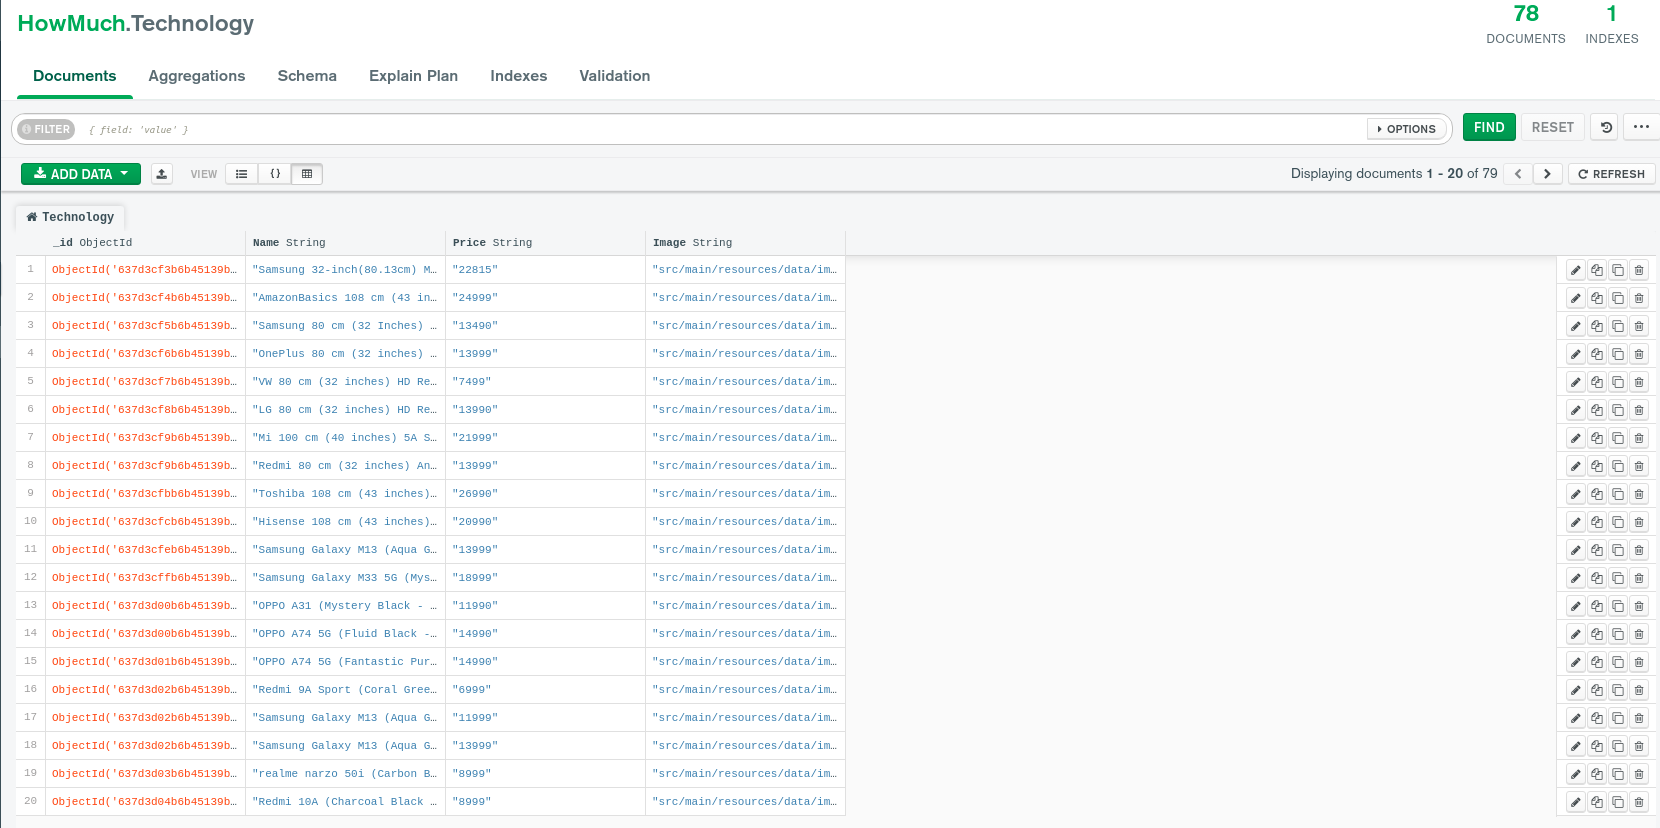
\includegraphics[scale=0.4]{mongo 1.png}
	\caption{A Screenshot of the MongoDB Compass Showing Records Stored in the Teachnology Schema}
\end{figure}

\begin{figure}[H]
	\centering
	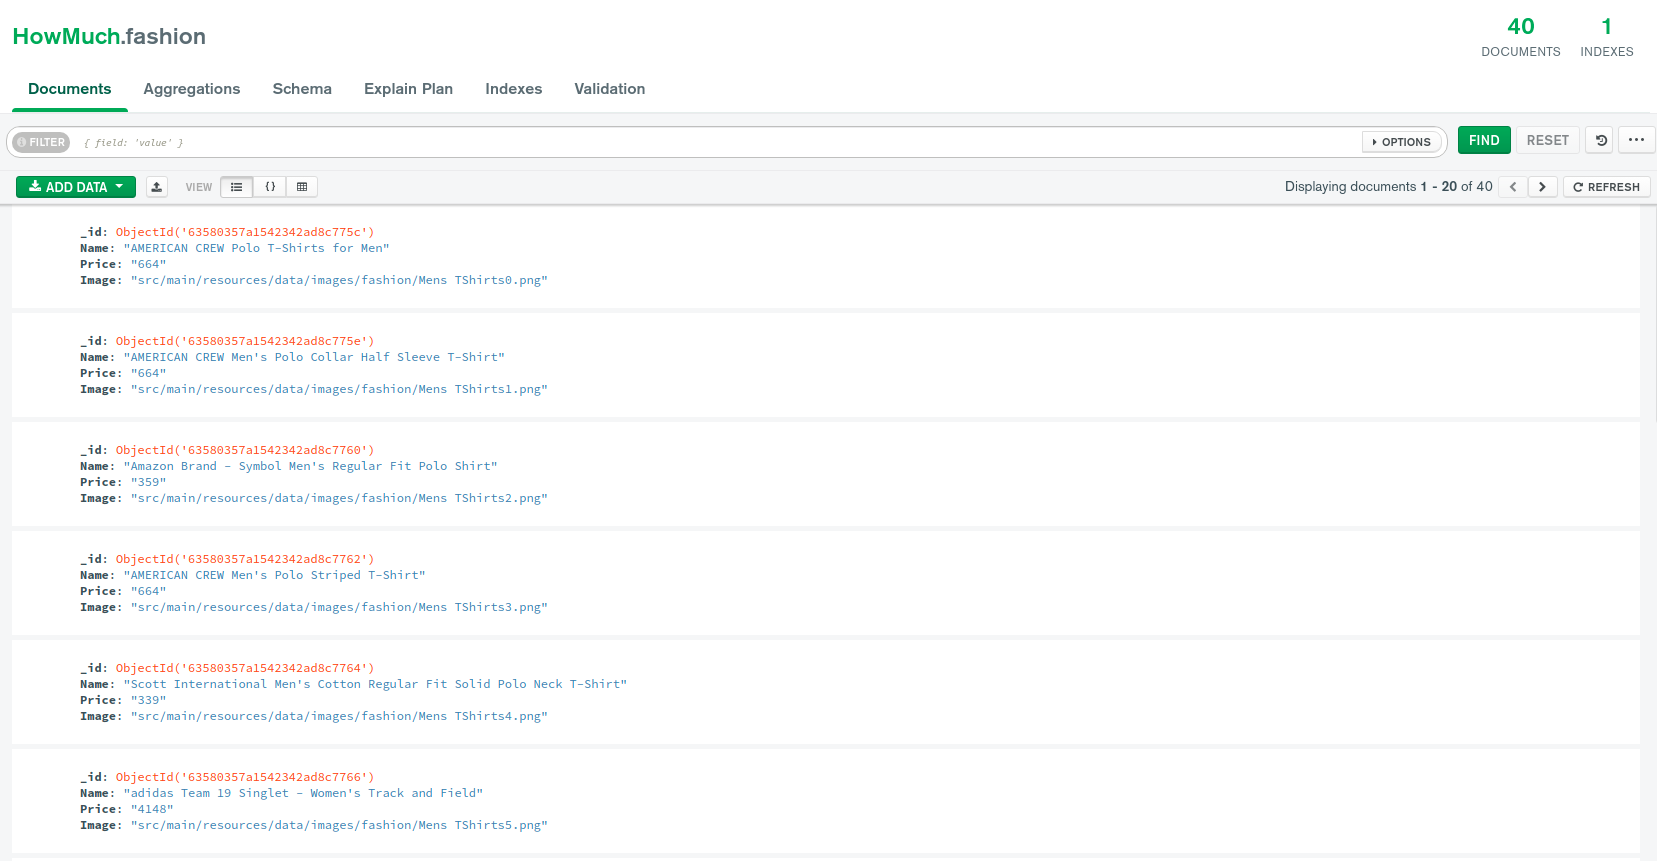
\includegraphics[scale=0.4]{mongo 2.png}
	\caption{Record Showing the Fashion Schema Documents}
\end{figure}
\subsection{Local CSV Files}
\begin{figure}[H]
	\centering
	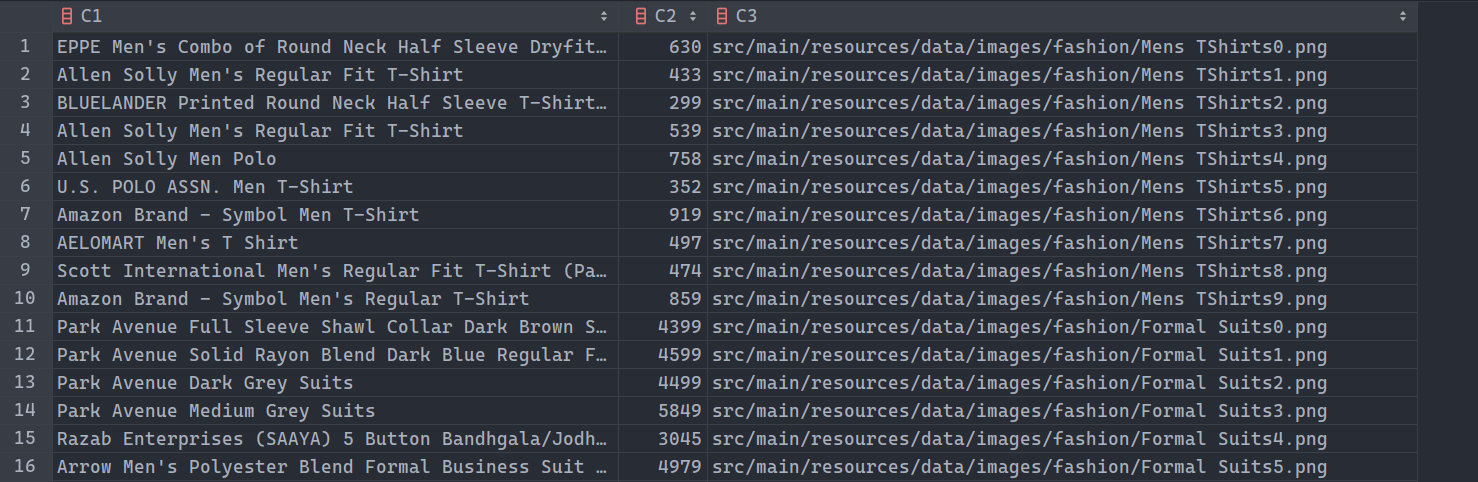
\includegraphics[scale=0.4]{csv.png}
	\caption{Screenshot of the Local CSV File}
\end{figure}
\section{Unique Features}
\subsection{Dark Mode}
Dark mode is toggled by a switch. It simply flips a boolean variable statically defined in Colors.java. Other classes will then set Colors on their screens depending on this variable, for each Swing element in their Panel or Frame. 
\begin{figure}[H]
\centering

\includegraphics[scale=0.5]{dark mode2.png}
\caption{Dark mode Turned on}
\end{figure}

\begin{figure}[H]
\centering

\includegraphics[scale=0.5]{dark mode1.png}
\caption{Dark mode Turned Off}
\end{figure}
\subsection{Data Backup}
Data backup is an important feature that ensures the user never has to face a situation where there is no product to be loaded on the Screen. 
\begin{itemize}
	\item There are 3 Databases maintained. 
	\item When updating, the program updates MongoDB and CSV if they have not been updated. 
	\item Each of the database have their own text file to maintain when the last time it was that they got updated. 
	\item They are updated only once a day, as updating takes time. 
	\item Updating is done in separate threads running in the Background. 
	\item There is a 3rd backup database of CSV files that just duplicates the current state of the CSV database each time the user exits the program. 
	\item The Game can update the Database in the Background while the user is playing the game, and at this point the backup database can be used. 
\end{itemize}
\subsection{Web Scrapping}
\begin{figure}[H]
\centering
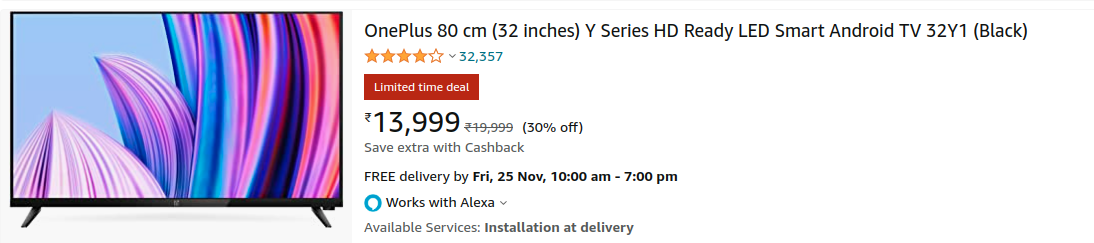
\includegraphics[scale=0.5]{amazon.png}
\caption{Product on Amazon}
\end{figure}

\begin{itemize}
	\item Every Webpage on amazon with some product has products that look like the one above.
	\item The HTML page is scrapped, and the respective divs are searched in it to find each product and its price. 
	\item It is then stored in the database after downloading and parsing the HTML file. 
\end{itemize}

\subsection{Working Login and Account Creation}
\begin{figure}[H]
\centering
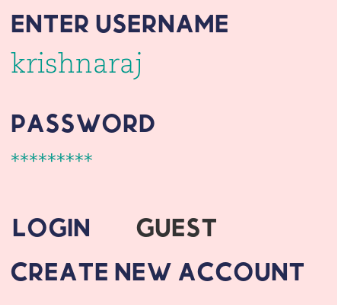
\includegraphics[scale=0.6]{login.png}
\caption{}
\end{figure}

\begin{itemize}
	\item All the Requirements of a simple login are satisfied here. 
	\item After the user inputs the username, it is valided in the local CSV file. 
	\item If found, the password is expected, checked and login is permitted. 
	\item If not found, password is validated, and a new user account creation is permitted. 
\end{itemize}

\section{Color Schemes Used}
\begin{figure}[H]
\centering
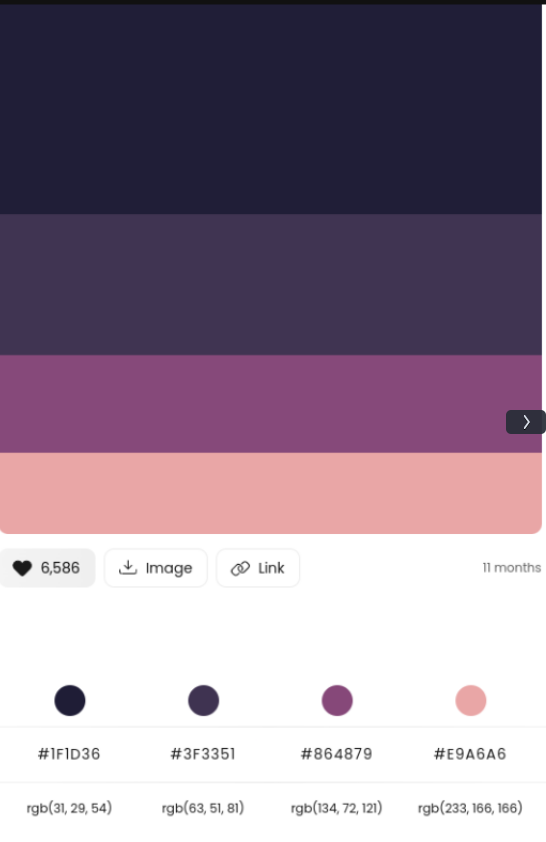
\includegraphics[scale=0.3]{design/Dark Mode Palette.png}
\caption{Color Palette}
\end{figure}
The Above Colors where used and are defined in the Colors.java.

\section{Screenshots of the Project}

\subsection{The Login Page}
\begin{figure}[H]
	\centering
	
\includegraphics[scale=0.45]{./design/Screenshots/Login Screen.png}
	\caption{The Login page after a successful login}
\end{figure}
\subsection{The Menu Screen}
\begin{figure}[H]
	\centering
	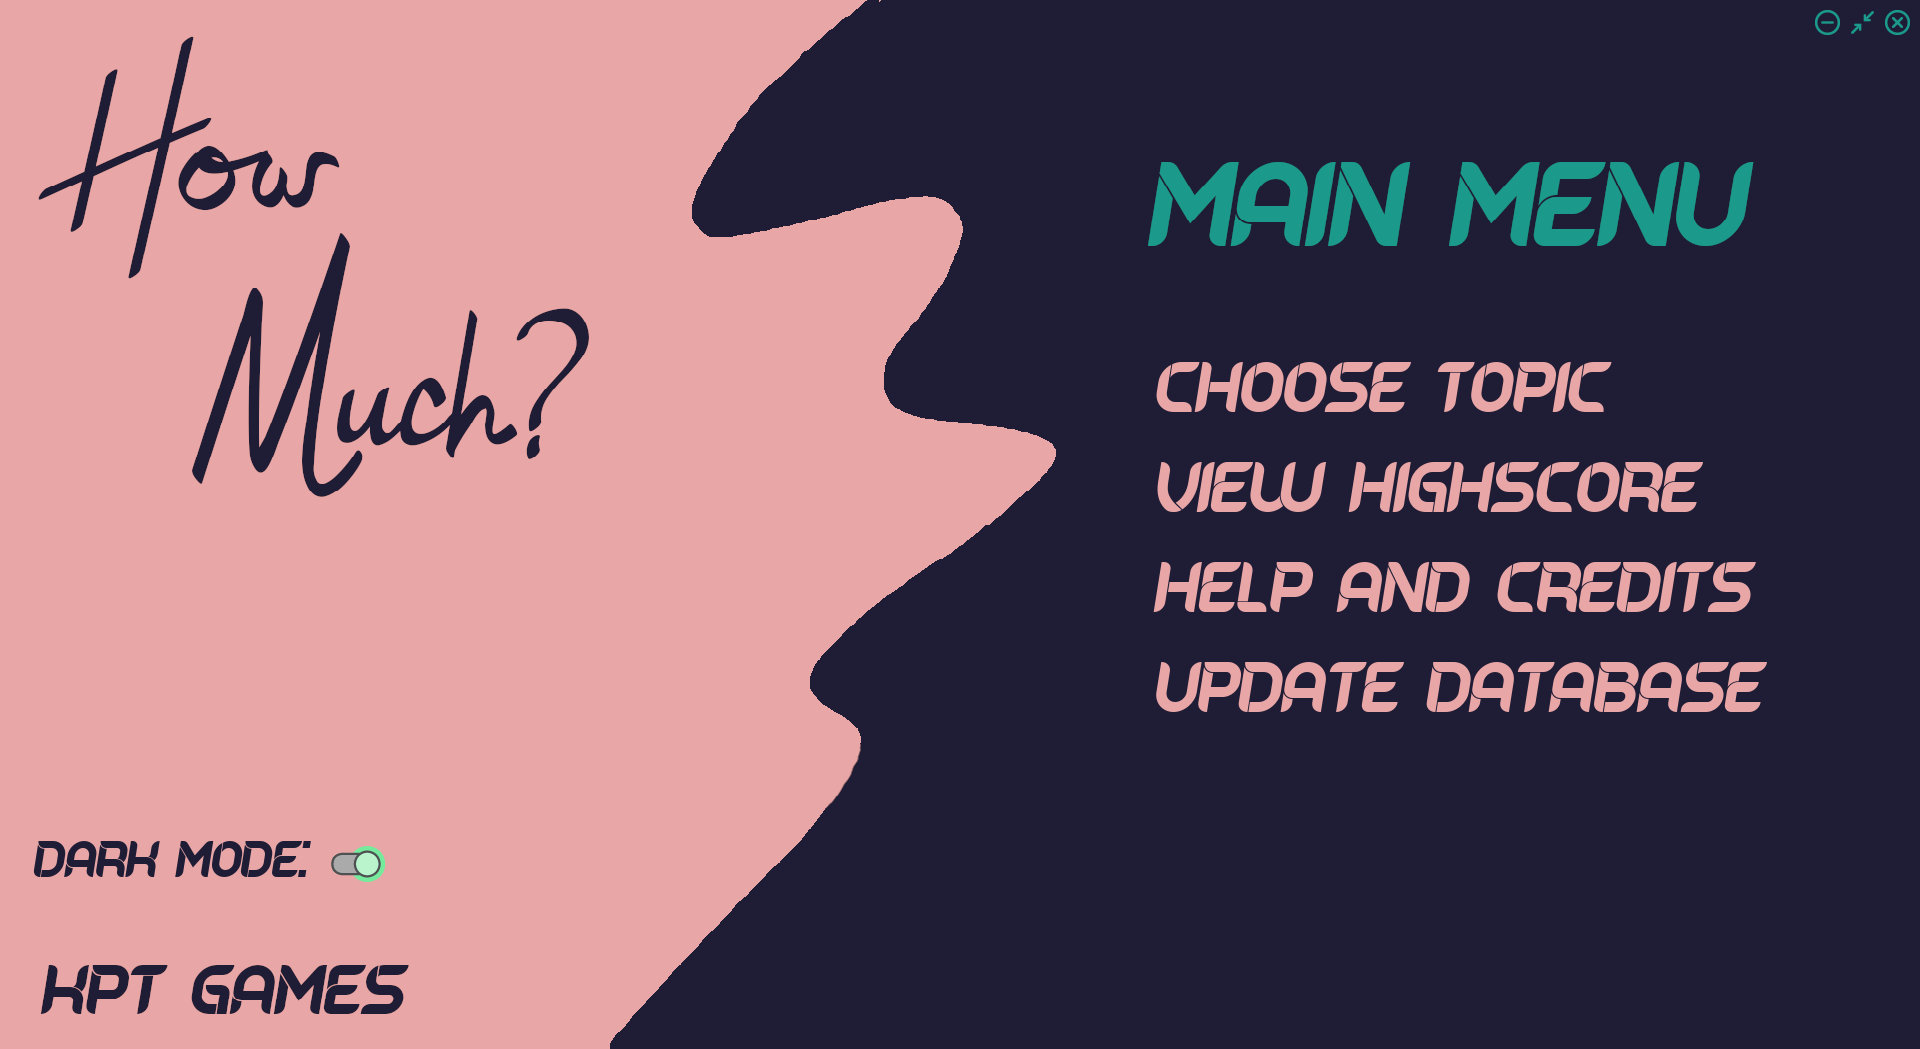
\includegraphics[scale=0.30]{./design/Screenshots/Main Menu Screen.png}
	\caption{}
\end{figure}


\subsection{The Topic Selection Screen}
\begin{figure}[H]
	\centering
	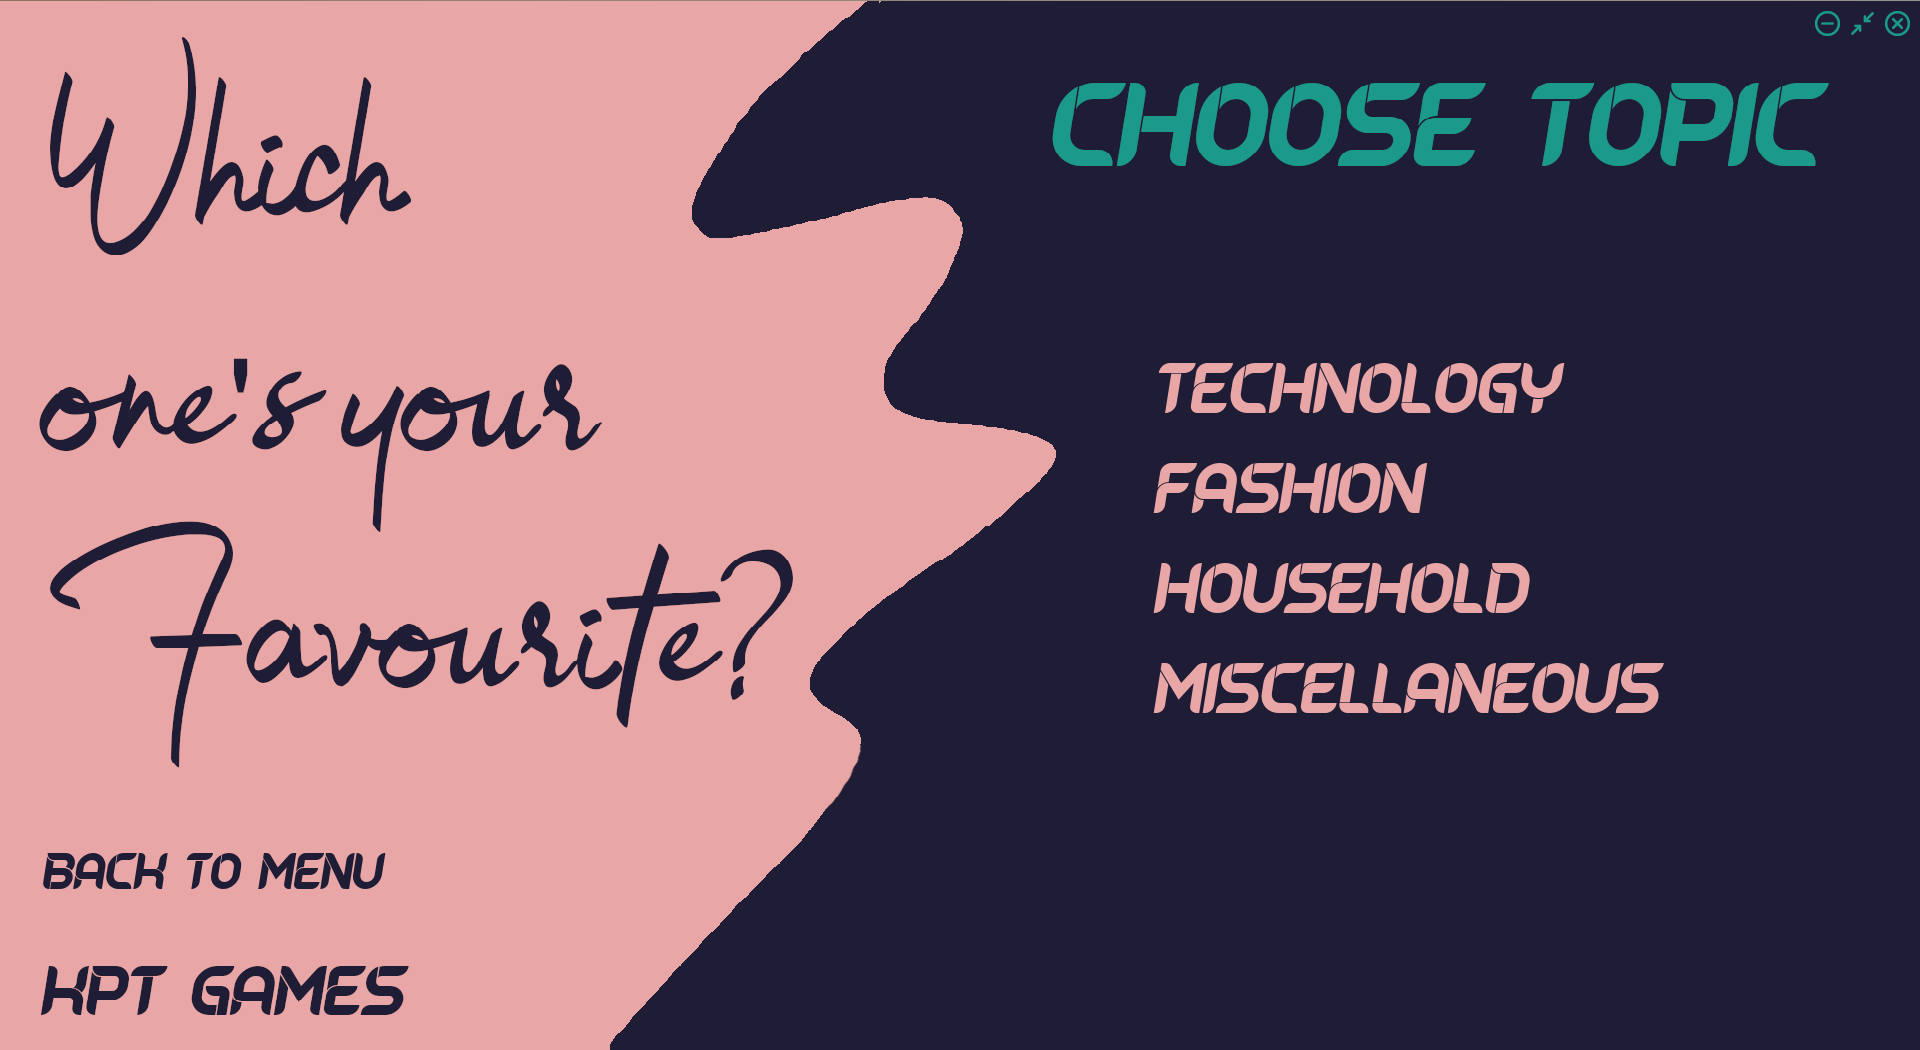
\includegraphics[scale=0.30]{./design/Screenshots/Topic Selection.png}
	\caption{The Login page after a successful login}
\end{figure}
\subsection{The Highscore Screen}
\begin{figure}[H]
	\centering
	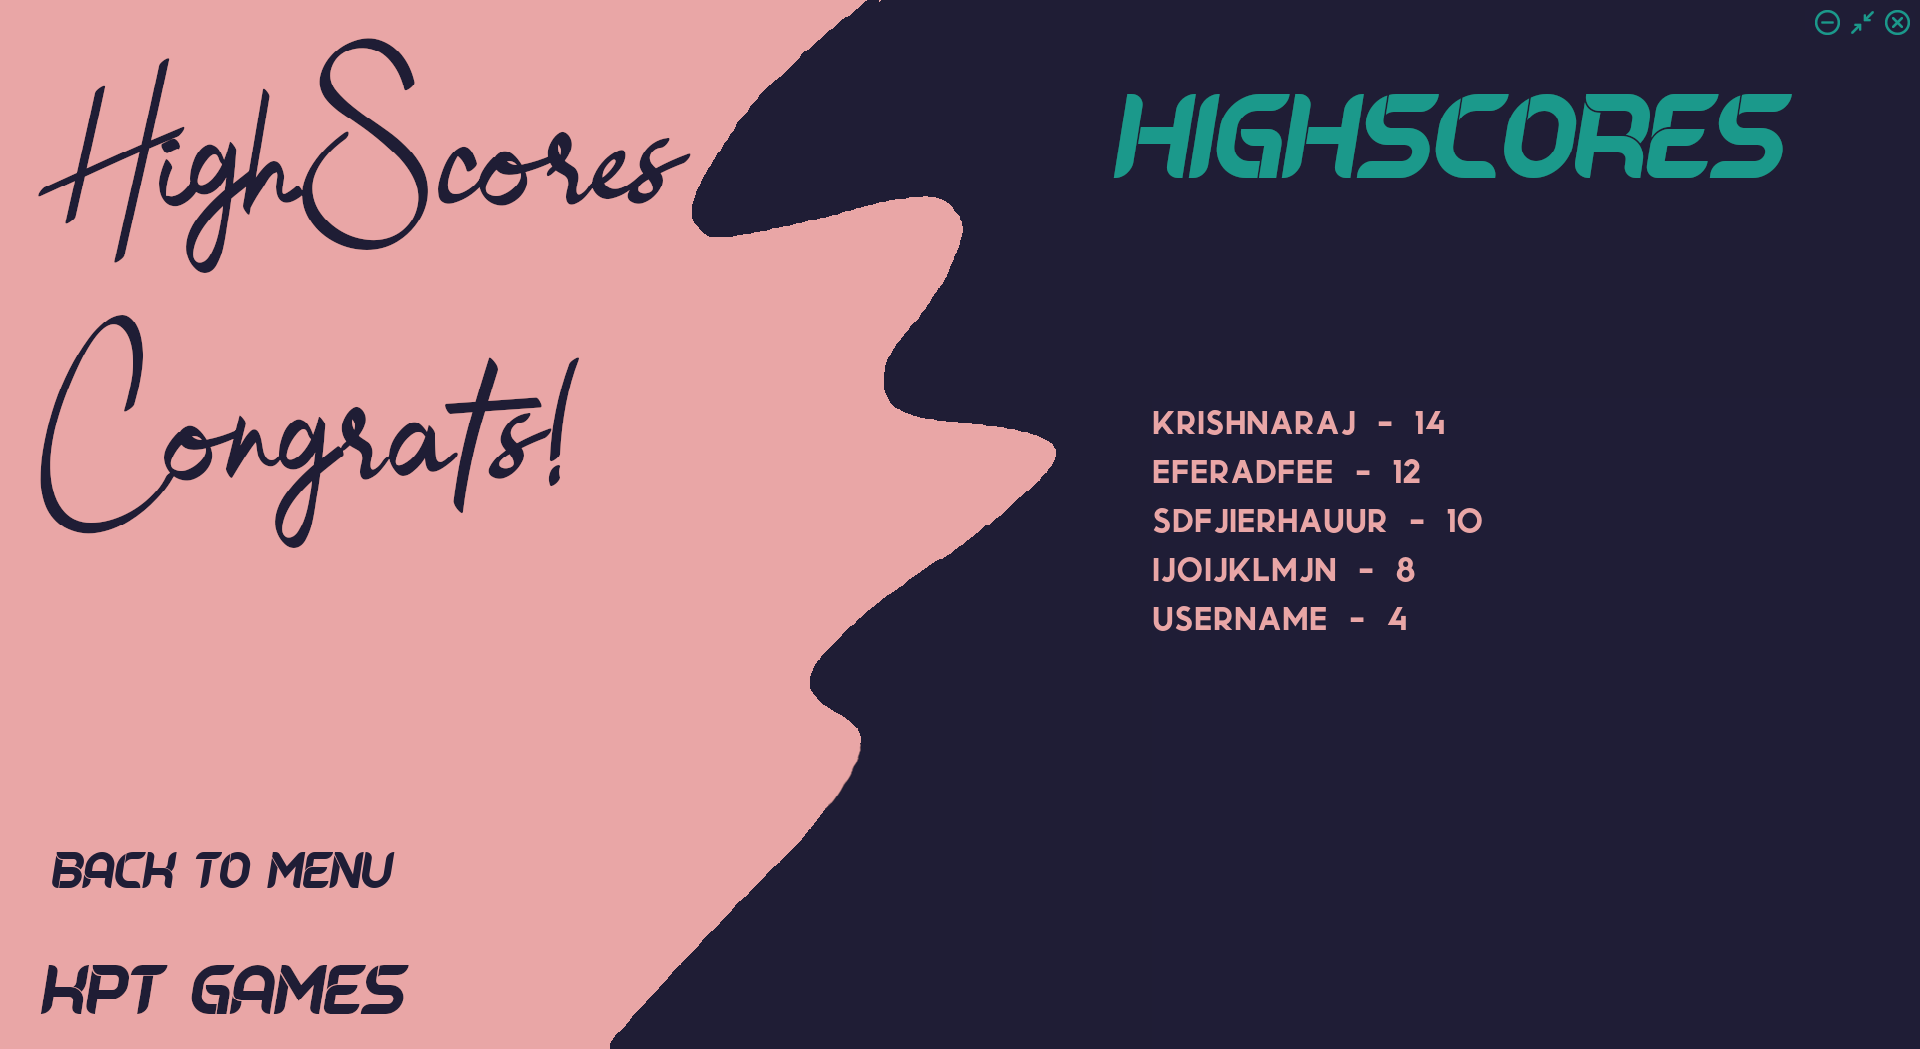
\includegraphics[scale=0.30]{./design/Screenshots/Highscores.png}
	\caption{The Login page after a successful login}
\end{figure}
\subsection{The Help and About}
\begin{figure}[H]
	\centering
	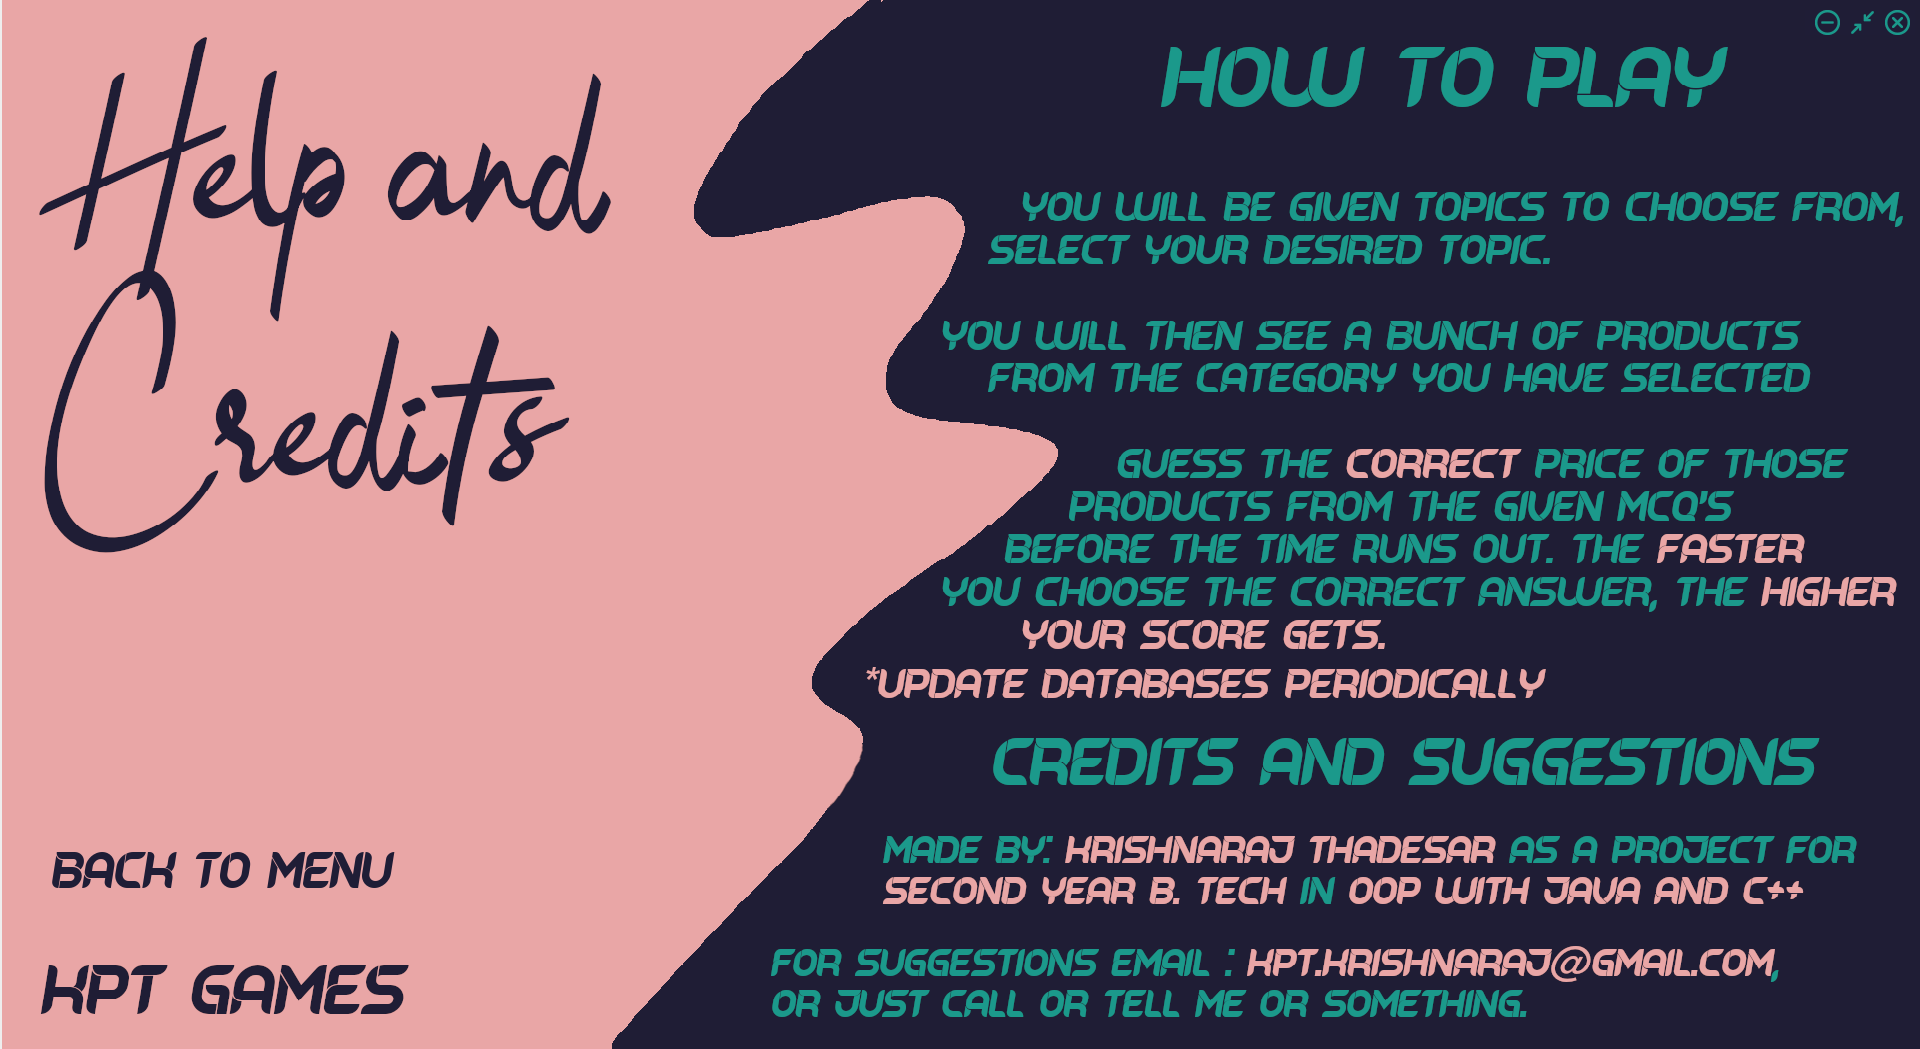
\includegraphics[scale=0.30]{./design/Screenshots/Help and Credits.png}
	\caption{The Login page after a successful login}
\end{figure}
\subsection{The Game Over Screen}
\begin{figure}[H]
	\centering
	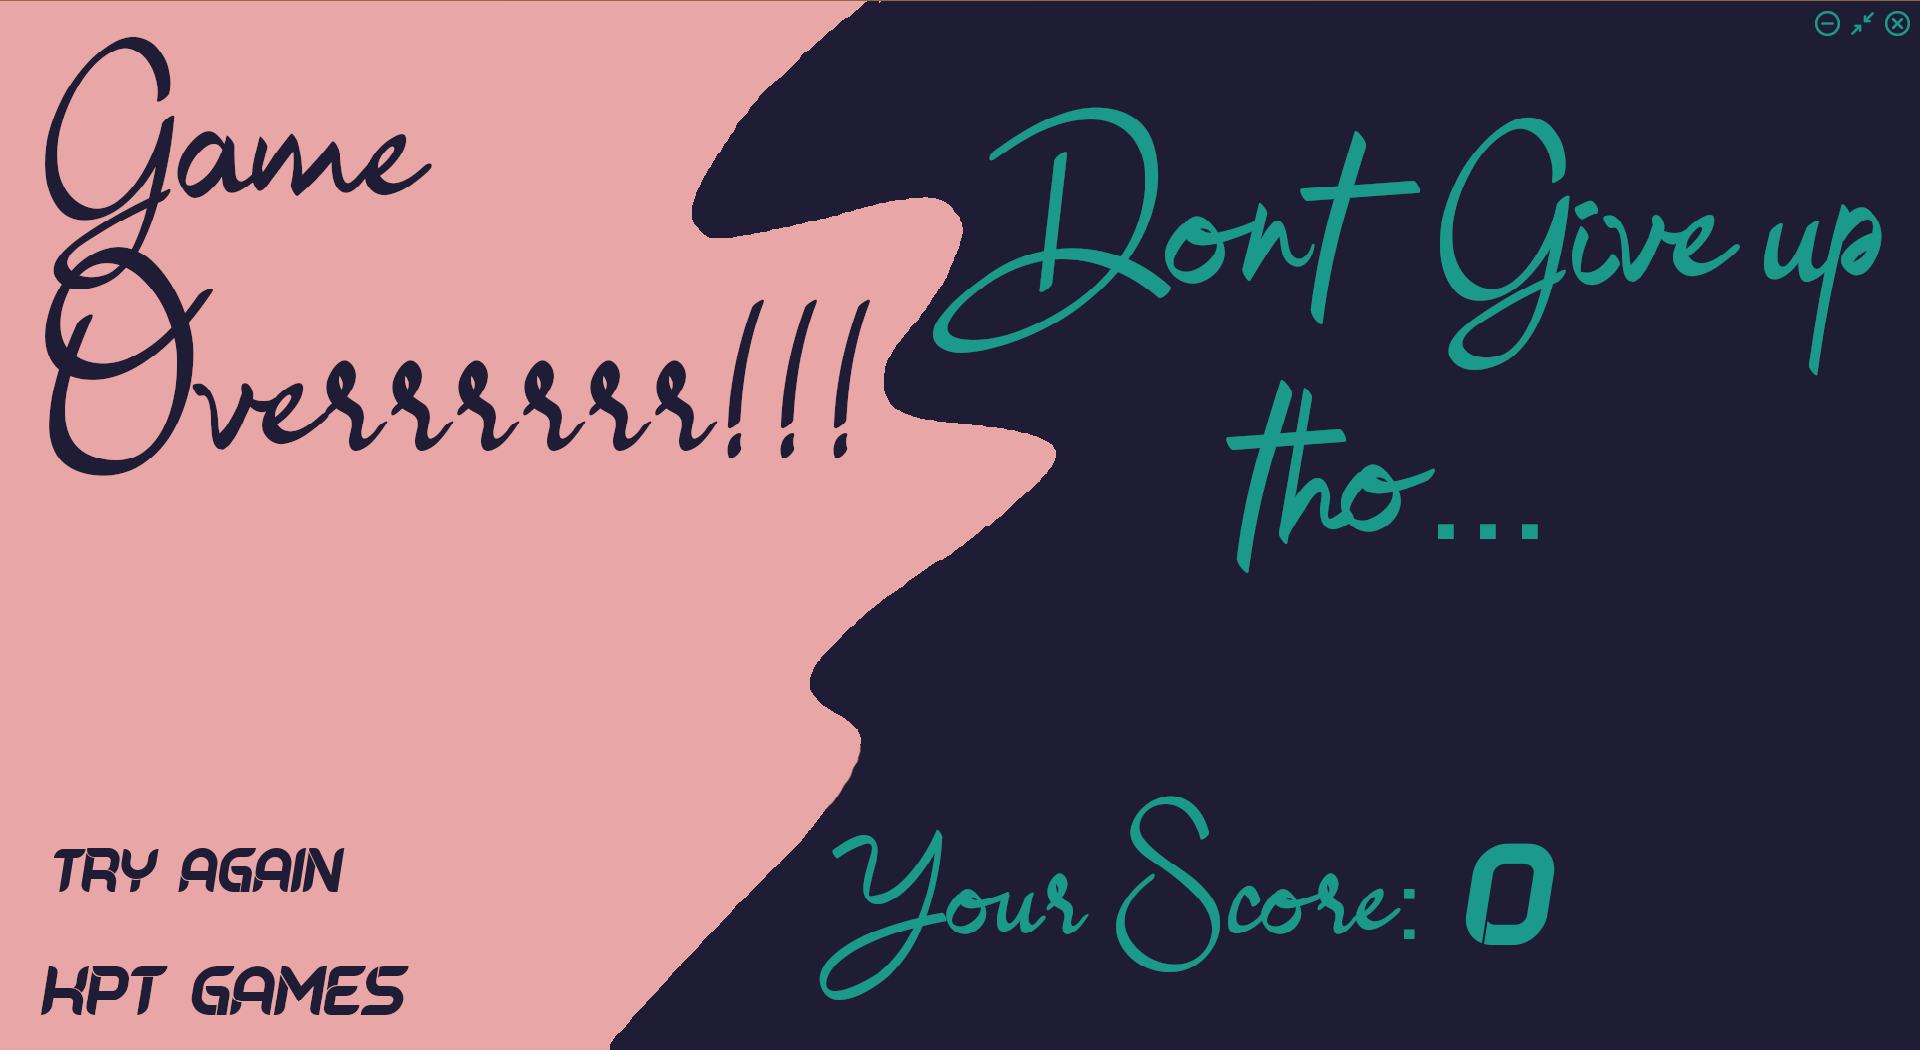
\includegraphics[scale=0.30]{./design/Screenshots/Game Over.png}
	\caption{The Login page after a successful login}
\end{figure}

\section{Walk-Through of the Files}

\subsection{Project Structure}
\begin{figure}[H]
	\centering
	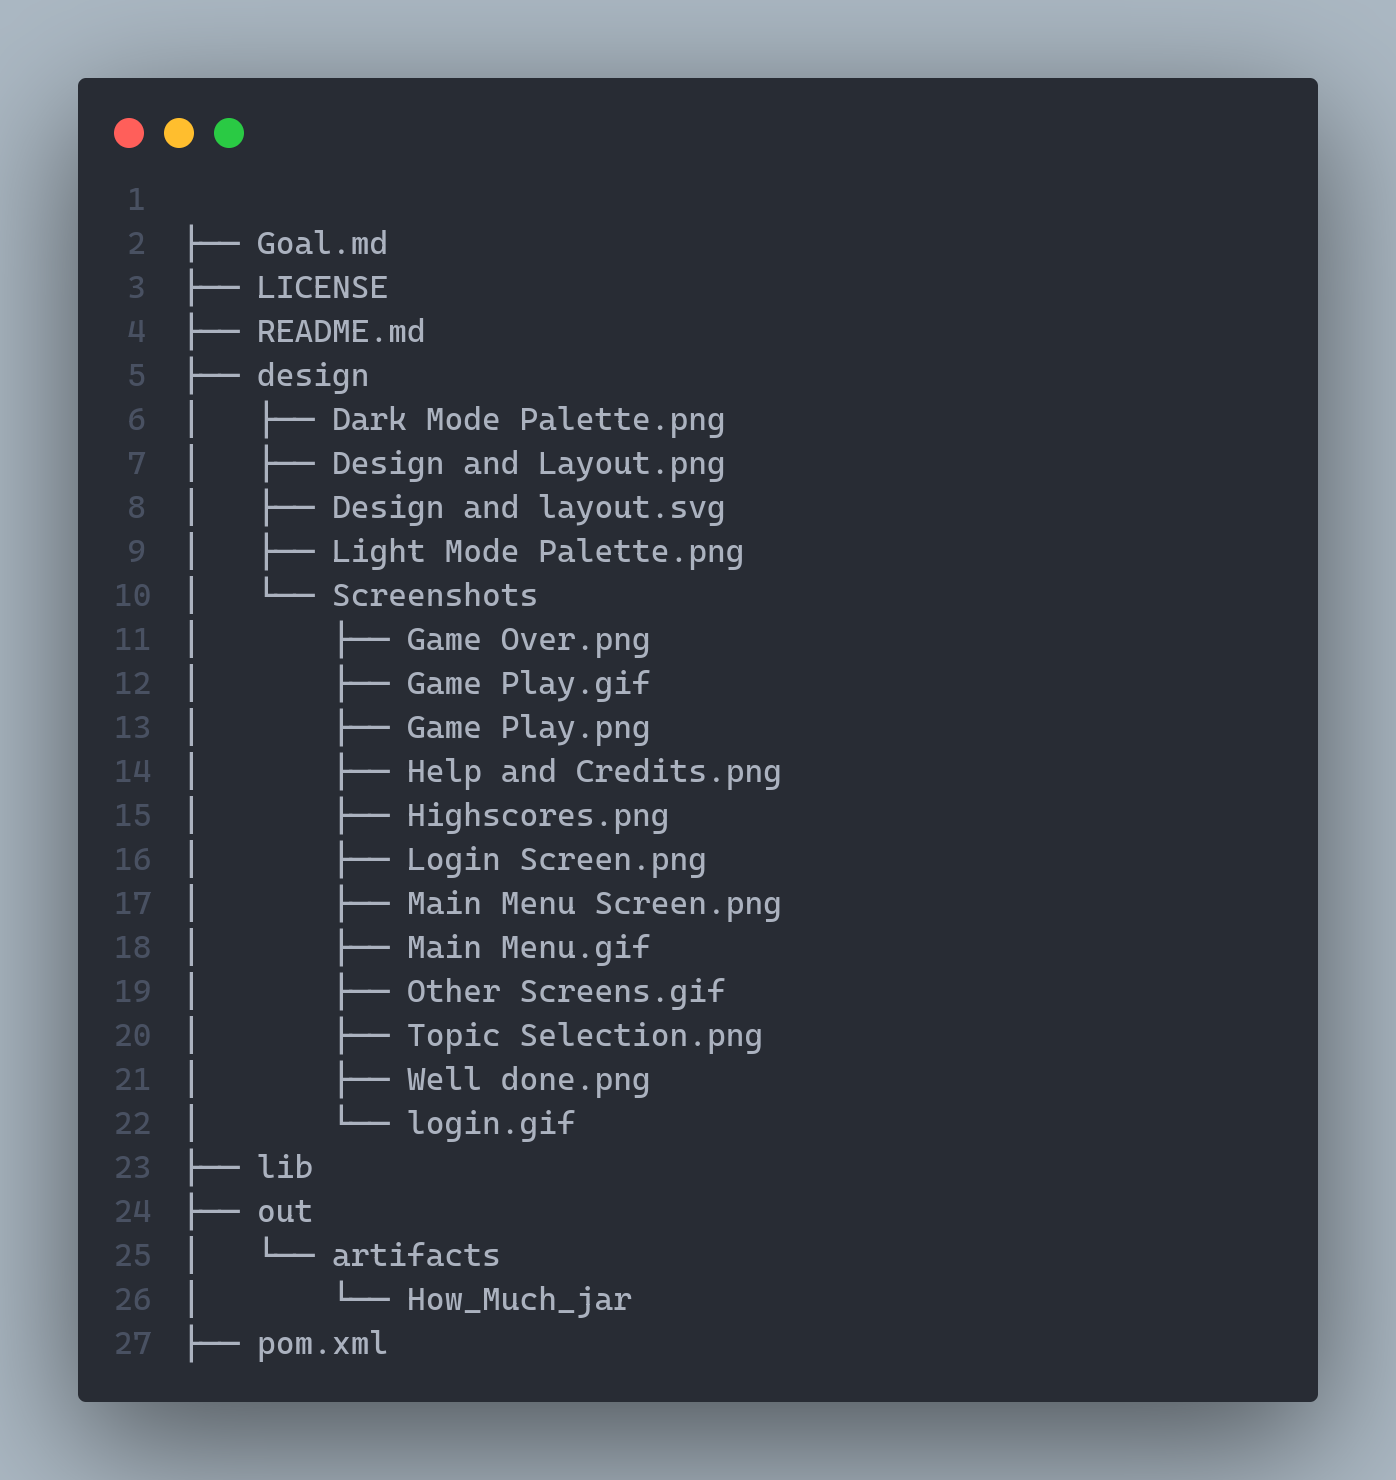
\includegraphics[scale=0.3]{code.png}
	\caption{}
\end{figure}
\begin{figure}[H]
	\centering
	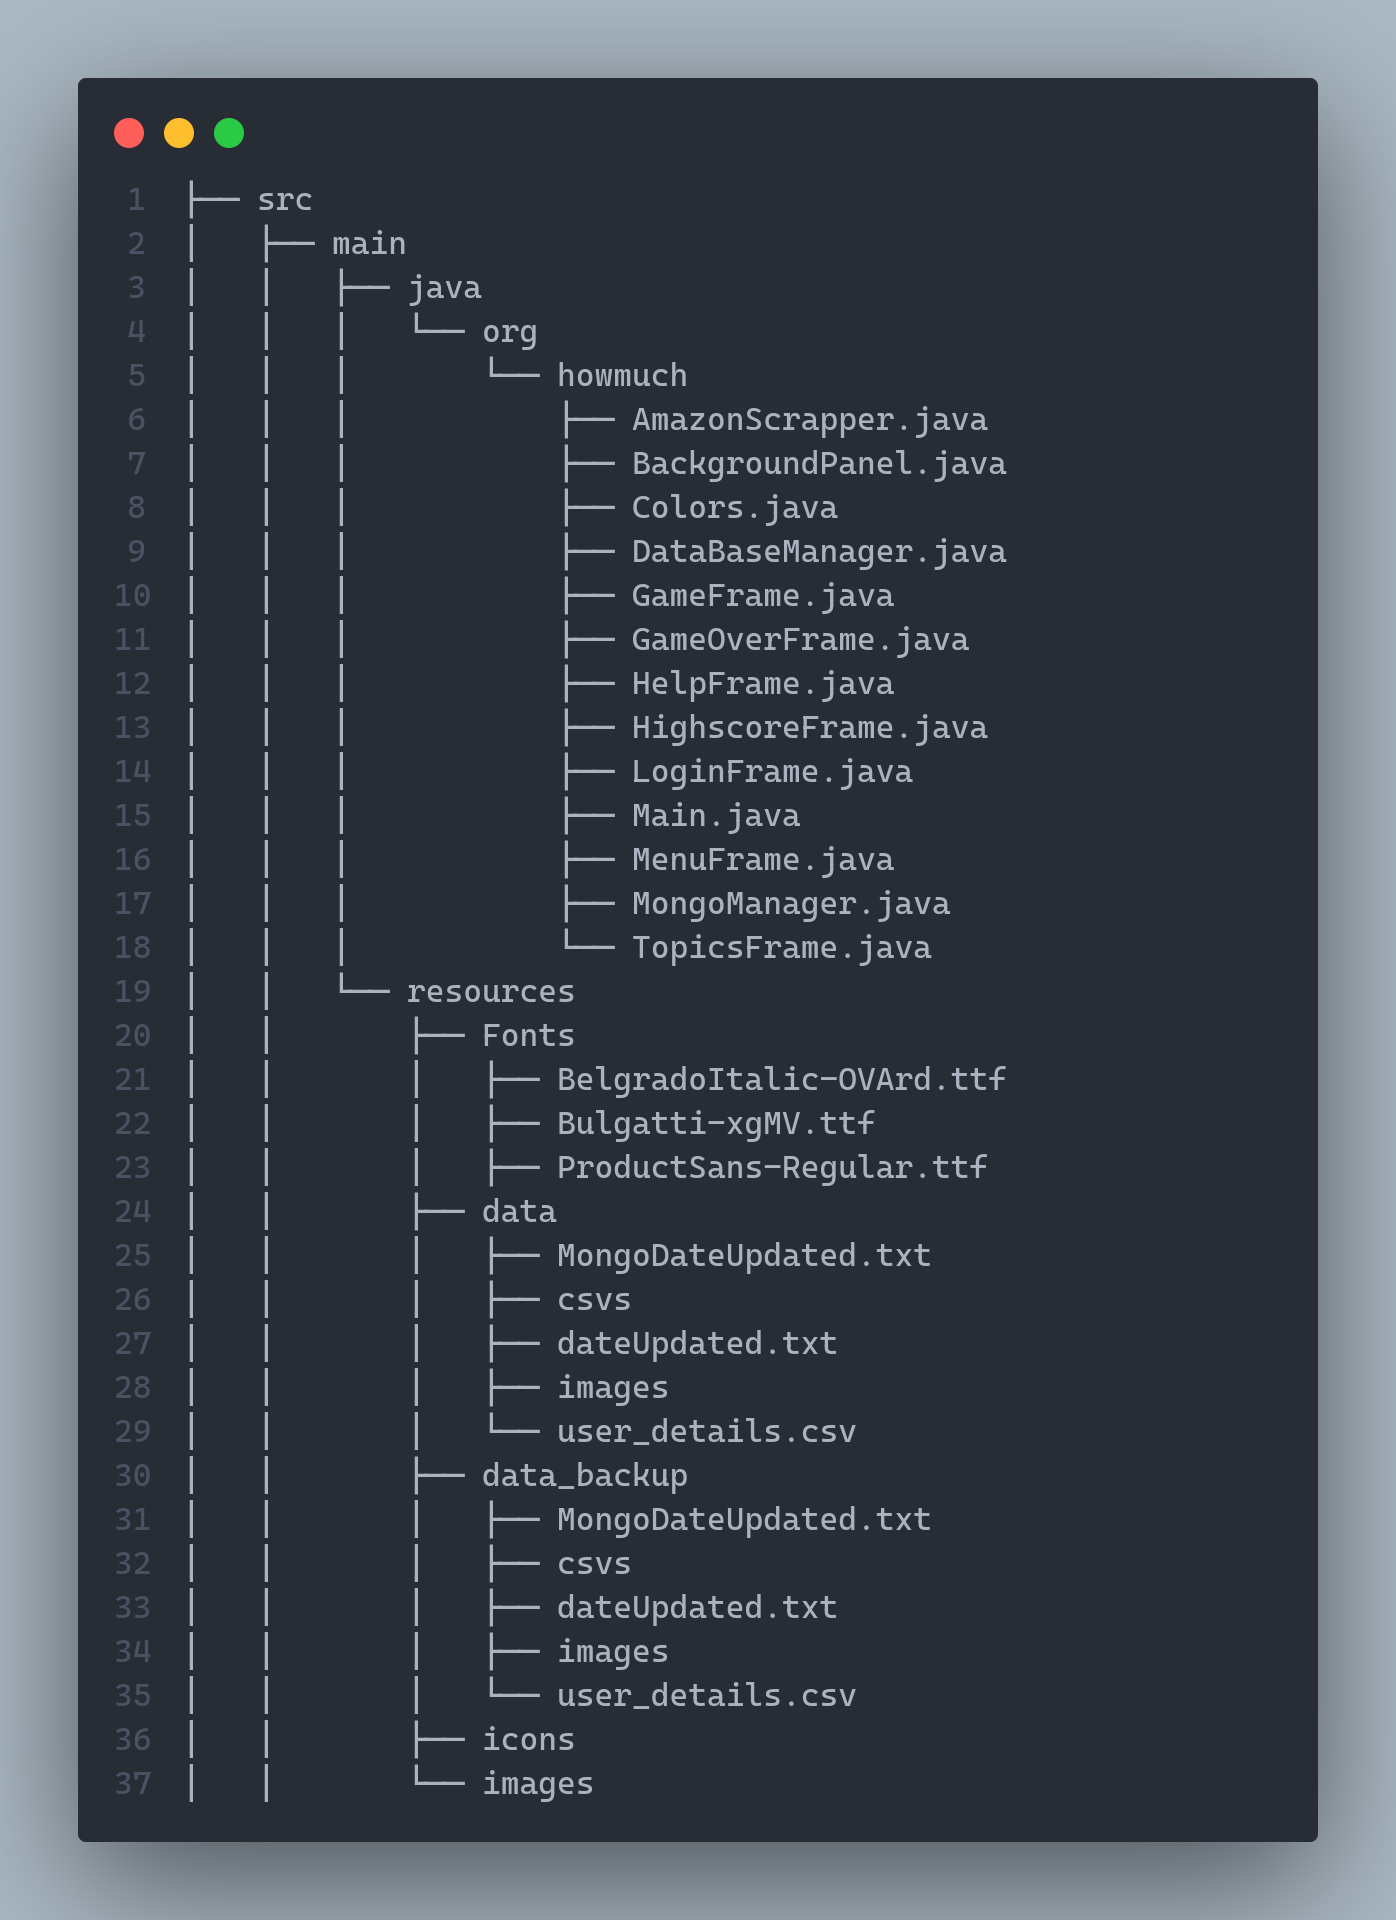
\includegraphics[scale=0.3]{code2.png}
	\caption{}
\end{figure}
\subsection{TopicsFrame.java}
This file manages the entire topic selection screen. It has various functions regarding showing the topics on the screen. It then sets static variables defined in the Main class with respect to the selected Topic. 
\subsection{MongoManager.java}
Important Class, which manages all interactions with Mongodb. It establishes connection with it, and flips a statically defined variable in Main called usingMongo to true or false depending on the success of the connection. It also has functions to update, clear, and retrieve values to and from the Mongo Database. 
\subsection{MenuFrame.java}
This file manages the entire Menu selection screen. It has various functions regarding showing the topics on the screen. It then sets static variables defined in the Main class with respect to the selected Topic.
It also has the Dark mode toggle, which flips a boolean called usingDarkMode defined in Colors.java. 

\subsection{Main.java}
This class calls all the other classes. It also has the main function. It uses multithreading to update the database at the same time as displaying the GUI. It has a function that manages the interactions between all the other classes. It also has several statically defined variables. 

\subsection{LoginFrame.java}
A Class that manages everything defined in the Login Screen. It has functions to check if the password fits the given criteria, and it queries and updates the database using functions defined in other classes.

\subsection{HighscoreFrame.java}
A Simple class that just displays the High scores of the User. It retrieves that data using database functions, and shows the top 5 Highscoring Users along with their scores. 
\subsection{HelpFrame.java}
A Simple Class that simply displays what to do in the game, how to play and the credits. 

\subsection{GameOverFrame.java}
A Simple class that just shows the score and gives an option to the user to go back to the main menu to try again if the game was lost, or won. 
\subsection{GameFrame.java}
This is the Main class, in that it shows the actual game. It has functions to check if the databases are working properly, and what to refer in case some of them dont work. It retrieves data using functions defind in other classes. Calculates 4 suitable options depending on the Correct price, and displayes everything on the Screen. 
\subsection{  DataBaseManager.java}
Important class that manages the Local CSV files. It updates, retrieves, and clears it. It also has functions to check the database for login functions, like password matching, username matching, adding username etc. 
\subsection{  Colors.java}
Another important class that has all the colors defined in it. It has a function to reassign colors, which is called every time the Dark Mode switch is flipped. 
\subsection{  BackgroundPanel.java}
Important class, as it is the panel that is used by all the other screens to display the background. It has a function to set the background as the Swing JPanel background by taking arguement of the location of the image to be inserted, while maintaining aspect ratio of the image. 

\subsection{  AmazonScrapper.java}
A very important class, as it has functions to actually scrap the data from amazon, and parse it. It then verifies the data, checks for invalid characters, and if everything is fine it calls functions from teh database class to insert new data into the databases. 

\section{Conclusion and Topics Learnt}
A lot of topics were learnt in the process of making this Project. It was very useful to make this Game, and it got me a lot more fluent in writing Java code.
\begin{enumerate}
	\item Multithreading was Understood in a greater depth, and implemented many times. 
	\item Web Scrapping was Learnt and in the process various java Libraries were used and understood.
	\item Swing in java was learnt in a higher detail.
	\item Database Management was understood. 
	\item JDBC Drivers, Connections of java with MongoDB and MySQL were learnt in detail. 
	\item Several Bugs were Resolved and as a Result of that programming skills were improved. 
	\item Designing skills were also improved.  
\end{enumerate} 
\section{Dependencies}

\lstinputlisting[language=xml, caption=Maven Dependency File]{/run/media/krishnaraj/Programs/Java/How Much/pom.xml}

\section{References}
\begin{itemize}
	\item https://www.notion.so/045f2a28abfe4a82a3ba0e8251c0e196?v=1ddbea2937324f79af4eae827f8a3132
	chrome://newtab/
	\item \url{https://classroom.google.com/u/0/w/NTUxMDUyMzM4MDk4/t/all}
	\item \url{https://webscraping.pro/scraping-amazon-webdriver-java/}
	\item \url{https://www.geeksforgeeks.org/scraping-amazon-product-information-using-beautiful-soup/}
	\item \url{https://www.scrapingbee.com/blog/web-scraping-amazon/}
	\item \url{https://docs.oracle.com/cd/E50453_01/doc.80/e50452/run_java_guis.htm#:~:text=In%20Java%20applications%2C%20the%20components,GUI%20forms%20can%20be%20built.}
	\item \url{https://www.javatpoint.com/multithreading-in-java}
	\item \url{https://www.digitalocean.com/community/tutorials/multithreading-in-java}
	\item \url{https://www.guru99.com/multithreading-java.html}
	\item \url{https://one.trustedstream.life/space-robot/?pl=uy-e9pFAkEqFCifo9sDBZw&sm=space-robot&hash=6IlUsQZL8I67jbxjdCa5gg&exp=1669365585}
	\item \url{https://www.mongodb.com/languages/java}
	\item \url{https://docs.oracle.com/javase/7/docs/api/javax/swing/package-summary.html#:~:text=The%20Action%20interface%20provides%20a,be%20accessed%20by%20several%20controls.&text=Defines%20the%20data%20model%20used,Slider%20s%20and%20ProgressBar%20s.}
	\item Credits to Teachers and Friends for their constant help and support.
\end{itemize}

\section{Code Files}

\lstinputlisting[language=Java, caption=Main Java File]{Colors.java}

\lstinputlisting[language=Java, caption=Main Java file]{BackgroundPanel.java}

\lstinputlisting[language=Java, caption=Main Java file]{Main.java}

\lstinputlisting[language=Java, caption=Main Java file]{LoginFrame.java}

\lstinputlisting[language=Java, caption=Main Java file]{GameFrame.java}

\lstinputlisting[language=Java, caption=Main Java file]{TopicsFrame.java}

\lstinputlisting[language=Java, caption=Main Java file]{GameOverFrame.java}

\lstinputlisting[language=Java, caption=Main Java file]{MongoManager.java}

\lstinputlisting[language=Java, caption=Main Java file]{DataBaseManager.java}

\lstinputlisting[language=Java, caption=Main Java file]{HighscoreFrame.java}

\lstinputlisting[language=Java, caption=Main Java file]{HelpFrame.java}

\lstinputlisting[language=Java, caption=Main Java file]{AmazonScrapper.java}



\end{document}